\subsection{PCA}
In order to do the PCA analyse some class had to be made for the dataset. The months was chosen as classes for trying to project the data in aspect of a year. 
By looking at PCA below the reader will see that around 90\% of the information is in component 1, of the PCA model. By this we can conclude that most of the variance happens in the first component and there by is the most important component. 

\vspace{-5pt}
\begin{figure}[!ht]
	\centering
	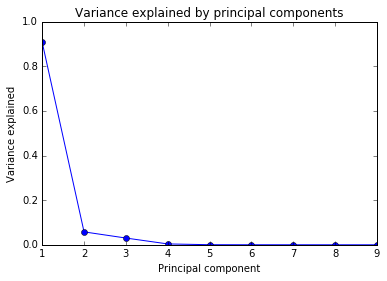
\includegraphics[width=0.7\textwidth]{fig/pca/pca_2.png}
	\vspace{-5pt}
\end{figure}